% "{'classe':('PSI'),'chapitre':'cin_point','type':('application'),'titre':'Étude des performances cinématiques en virage d’une Formule 1', 'source':'Florestan Mathurin','comp':(''),'corrige':True}"
%\setchapterimage{fig_00.jpg}
\chapter*{Application \arabic{cptApplication} \\ 
Étude des performances cinématiques en virage d’une Formule 1 -- \ifprof Corrigé \else Sujet \fi}
\addcontentsline{toc}{section}{Application \arabic{cptApplication} : 
Étude des performances cinématiques en virage d’une Formule 1 -- \ifprof Corrigé \else Sujet \fi}

\iflivret \stepcounter{cptApplication} \else
\ifprof  \stepcounter{cptApplication} \else \fi
\fi

\setcounter{question}{0}

\marginnote{Ressources de Florestan Mathurin.}
\marginnote[1cm]{
%\UPSTIcompetence[2]{B2-14}
%\UPSTIcompetence[2]{C1-05}
%\UPSTIcompetence[2]{C2-07}
}


\begin{marginfigure}
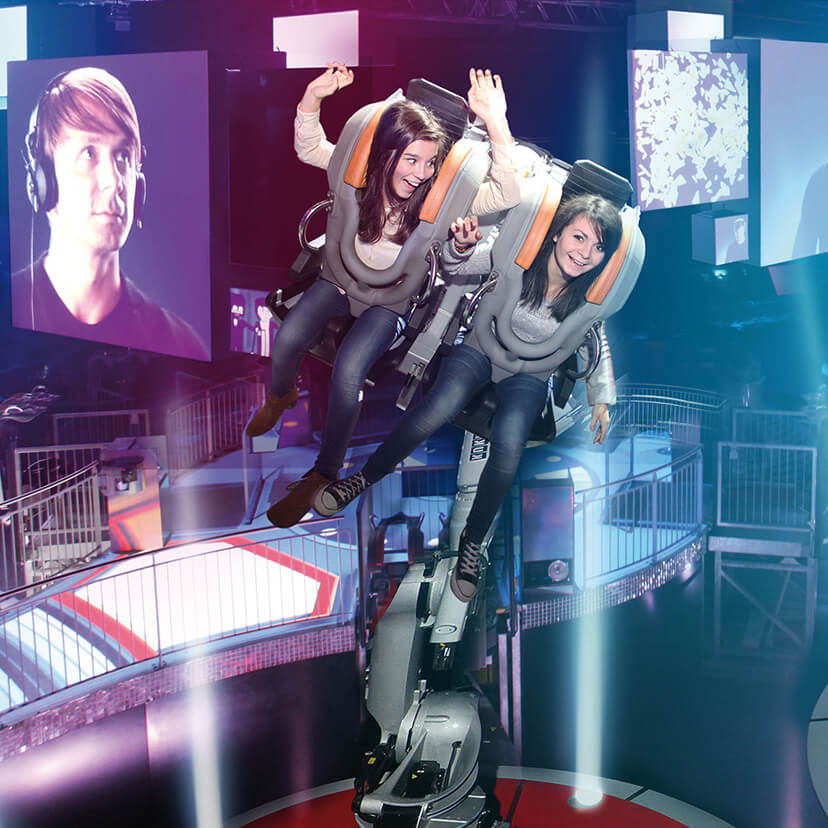
\includegraphics[width=\linewidth]{fig_01}
\end{marginfigure}




\begin{center}
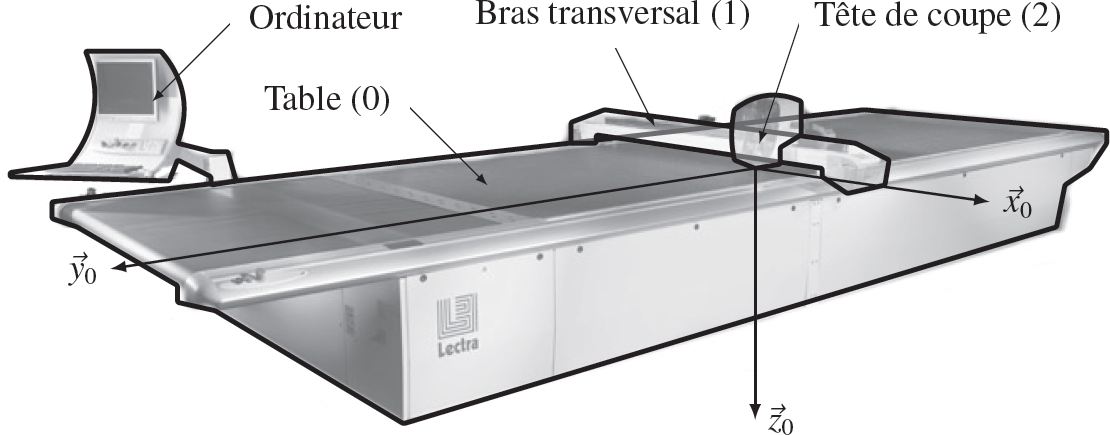
\includegraphics[width=\linewidth]{fig_02}
%\textit{}
\end{center}



\subsection*{Mise en situation}
Une Formule 1 doit assurer un certain nombre d’exigences techniques afin d’assurer les meilleures performances en course tout en garantissant la sécurité du pilote. Une de ces exigences est que « le système doit tenir la trajectoire en phase de virage ». Pour y parvenir, le véhicule dispose d'une cinématique particulière permettant aux roues de tourner sur le sol en limitant le risque de glissement. On s'intéresse aux conséquences pratiques nécessaire pour assurer la condition de roulement sans glissement des roues sur le sol. On supposera donc que les 4 roues roulent sans glisser dans le plan
$\left(O,\vect{x_0},\vect{y_0}\right)$. 


Pour cette étude on considère que le véhicule est constitué d’un châssis \textbf{$(S)$} et de 4 roues \textbf{$(S_i)$}
 avec $i=1,2,3,4$.  Le châssis est modélisé par un rectangle $A_1A_2A_3A_4$ tel que 
 $\vect{A_4 A_3}=\vect{A_1 A_2}=2d\vect{x}$ et $\vect{A_4 A_1}=\vect{A_3 A_2}=L\vect{y}$  où $L$ correspond à l’empattement du véhicule et $2d$ à la voie. 


On définit le repère $\rep{}\repere{C}{x}{y}{z}$ attaché au châssis où le point $C$, origine du repère, est tel que 
$\vect{A_4 C}= d\vect{x}$. Le véhicule est en phase de virage et on considère alors qu’il est en rotation par rapport au
repère $\rep{0}\repere{O}{x_0}{y_0}{z_0}$ autour du point $I_{S/R0} = I$, centre instantanée de rotation du mouvement. On pose $\beta=\angl{x_0}{x}$  angle de rotation du châssis par rapport à $\rep{0}$. 

On définit le repère $\rep{i}\repere{A_i}{u_i}{p_i}{q_i}$ attaché à chaque roue $(S_i)$ . Ces 4 roues de rayon $R$ sont en
liaison pivot avec le châssis $(S)$ suivant les axes $\axe{A_i}{u_i}$ avec 
$i=1,2,3,4$. On pose $\theta_i=\angl{z}{q_i}$ angle de rotation de la roue $i$ par rapport au châssis. 
Afin d’assurer la direction du véhicule, les 2 roues pivotent d’un angle $\psi_1$ suivant l’axe $\axe{A_i}{z}$ pour la roue 1 et d’un angle $\psi_2$ suivant l’axe $\axe{A_2}{z}$) pour la roue 2 avec $\psi_1=\angl{x}{u_1}=\angl{y}{v_1}$ et $\psi_2=\angl{x}{u_2}=\angl{y}{v_2}$. 
On considère que le contact sol/roue et assimilable à un contact ponctuel en $I$ de normale $\axe{I}{z}$ tel que $\vect{I_i A_i}=R\vect{z}$ .  



\question{Établir les figures géométrales utiles.}
\ifprof%
\begin{corrige}
\end{corrige}\else\fi

\question{Écrire la condition de roulement sans glissement de la roue $(S_1)$ par rapport au sol $\rep{0}$. En déduire une relation vectorielle simple entre $\vectv{I_1}{S_1}{S}$ et $\vectv{I_1}{S}{\rep{0}}$.}
\ifprof%
\begin{corrige}
\end{corrige}\else\fi

\question{Donner la forme simple du torseur cinématique $\torseurcin{V}{S}{\rep{0}}$ écrit en $I$. En déduire alors $\vectv{I_1}{S}{\rep{0}}$ en fonction de $\vecto{S}{\rep{0}}$ et $\vect{II_1}$ (on n'effectuera pas les produits vectoriels).}
\ifprof%
\begin{corrige}
\end{corrige}\else\fi

\question{Donner la forme simple du torseur cinématique $\torseurcin{V}{S_1}{S}$ écrit en $A_1$. En déduire alors $\vectv{I_1}{S_1}{S}$ en fonction de $\vecto{S_1}{S}$ et $\vect{A_1 I_1}$ (on n'effectuera pas les produits vectoriels).}
\ifprof%
\begin{corrige}
\end{corrige}\else\fi

\question{Déduire des relations précédentes que $\vecto{S}{\rep{0}}\wedge \vect{IA_1} + \vecto{S_1}{\rep{0}}\wedge \vect{A_1I_1}=\vect{0}$.}
\ifprof%
\begin{corrige}
\end{corrige}\else\fi

\question{On pose $\vect{IA_1}=a\vect{u_1}+b\vect{v_1}+c\vect{z}$, montrer que l'on a nécessairement $a=-\dfrac{R\dot{\theta}_1}{\dot{\beta}}$ et $b = 0$ pour que la relation obtenue question précédente soit respectée. }
\ifprof%
\begin{corrige}
\end{corrige}\else\fi

\question{Montrer que l'axe $(D_1)$ de la roue $(S_1)$ passe par $I$,  puis en déduire que l'axe $(D_i )$ de la roue $(S_i )$ passe par $I$.}
\ifprof%
\begin{corrige}
\end{corrige}\else\fi


  On pose par la suite $\vect{IC}=\rho \vect{x}$ et on note $\vectv{C}{S}{R} =V\vect{y}$ ($\rho$ est le rayon du virage et $V$ la vitesse du véhicule).
  
\question{À partir de $\torseurcin{V}{S}{\rep{0}}$ exprimé en $I$, quelle relation simple existe-t-il entre $V$ et $\rho$ ?}
\ifprof%
\begin{corrige}
\end{corrige}\else\fi

\question{En utilisant les résultats de la question précédente, déterminer les vitesses de rotation $\dot{\theta}_3$ et $\dot{\theta}_4$ des deux roues arrières $(S_3)$ et $(S_4)$ en fonction de $\rho$, $R$, $d$ et $V$. Que constate-t-on ? }
\ifprof%
\begin{corrige}
\end{corrige}\else\fi

\question{En déduire une condition technologique à assurer sur l'essieu arrière pour que les conditions de roulement sans glissement soient respectées en $I_3$ et $I_4$. }
\ifprof%
\begin{corrige}
\end{corrige}\else\fi

On considère que le véhicule roule à \SI{90}{km}{h}, les roues ont pour diamètre \SI{80}{cm} et le virage décrit une courbe telle que la vitesse angulaire du véhicule  $\dot{\beta}=\SI{0,1}{rad/s}$. On donne $d=\SI{1}{m}$. 

\question{Déterminer graphiquement les vitesses des roues $S_1$, $S_2$, $S_3$, $S_4$ en $I_1$, $I_2$, $I_3$, $I_4$ . Utiliser une échelle judicieuse pour les vitesses et  justifier les constructions.}
\ifprof%
\begin{corrige}
\end{corrige}\else\fi

\question{Que constate-t-on sur les roues avants et en déduire une condition technologique à assurer sur l'essieu avant pour que les conditions de roulement sans glissement soient respectées en $I_1$ et $I_2$ . }
\ifprof%
\begin{corrige}
\end{corrige}\else\fi

